\documentclass[11pt]{article}

% ---------- packages ----------
\usepackage[a4paper,margin=18mm,top=16mm,bottom=18mm]{geometry}
\usepackage[T1]{fontenc}
\usepackage[default,scale=0.98]{sourcesanspro}
\usepackage{sourcecodepro}
\usepackage{microtype}
\usepackage{xcolor}
\usepackage{graphicx}
\usepackage{enumitem}
\usepackage{booktabs}
\usepackage{titlesec}
\usepackage{parskip}
\usepackage{pifont}
\usepackage[most]{tcolorbox}
\usepackage[hidelinks]{hyperref}

\graphicspath{{./}}

% ---------- palette ----------
\definecolor{brand}{HTML}{0D9488}
\definecolor{brandd}{HTML}{0F766E}
\definecolor{ink}{HTML}{0F172A}
\definecolor{slate}{HTML}{475569}
\definecolor{mist}{HTML}{F1F5F9}
\definecolor{rose}{HTML}{E11D48}
\definecolor{amber}{HTML}{B45309}
\definecolor{grn}{HTML}{047857}

\color{ink}

% ---------- section styling ----------
\titleformat{\section}
  {\color{brandd}\bfseries\large}{}{0pt}
  {\;}[{\color{brand!40}\titlerule[1pt]}]
\titlespacing*{\section}{0pt}{14pt}{6pt}

\setlist[itemize]{leftmargin=1.15em,itemsep=2.5pt,topsep=3pt}
\newcommand{\yes}{\textcolor{grn}{\ding{51}}\;}
\newcommand{\gap}{\textcolor{amber}{\ding{72}}\;}
\newcommand{\term}[1]{\textbf{#1}}

% ---------- card box ----------
\tcbset{
  card/.style={
    enhanced, breakable,
    colback=white, colframe=brand!35, boxrule=0.7pt, arc=3pt,
    left=9pt, right=9pt, top=7pt, bottom=7pt,
    fonttitle=\bfseries, coltitle=white,
    colbacktitle=brand, attach title to upper={\par\smallskip},
    title=#1
  },
  plaincard/.style={
    enhanced, breakable, colback=mist, colframe=mist,
    arc=3pt, left=9pt, right=9pt, top=7pt, bottom=7pt
  }
}

\setlength{\parskip}{4pt}
\pagestyle{empty}

% =====================================================================
\begin{document}

% ---------- title band ----------
\begin{tcolorbox}[enhanced, colback=ink, colframe=ink, arc=4pt,
  left=16pt, right=16pt, top=13pt, bottom=13pt, coltext=white]
  {\fontsize{24}{26}\selectfont\bfseries Encrypted\textcolor{brand}{-}Chaos}\\[3pt]
  {\large Teaching an AI to read encrypted pictures}\\[7pt]
  {\color{white!70}\small
  A bench that tests whether a neural network can rebuild an image from its
  scrambled (encrypted) version \textbf{without ever being given the password}.}\\[9pt]
  {\color{white!55}\footnotesize\ttfamily
  MS/PhD thesis MVP \textbullet\ Supervisor: Dr.\ Ayesha Khalid \textbullet\
  github.com/ali-Hamza817/Encrypted-Chaos}
\end{tcolorbox}

% ---------- the problem ----------
\section{The problem, in plain English}

Many apps protect images with \term{chaos-based encryption}: fast maths that scrambles
pixels using chaotic (wildly unpredictable) number sequences. It is popular because
full-strength encryption such as AES can be slow for large images.

These schemes are judged by \term{statistical tests}: does the scrambled image look like
random noise? does changing one bit of the key change the whole output? Almost every
published scheme passes.

\begin{tcolorbox}[plaincard]
\textbf{But passing those tests does not prove the scheme is safe against a modern
attacker who uses machine learning.} Instead of doing classical maths to recover the key,
such an attacker collects many \emph{(original image, encrypted image)} pairs and trains a
neural network to undo the encryption directly. Published work in 2019 and 2025 showed this
can work. The open questions: how far does it go? Does it still work on keys or schemes the
network never saw? How does it compare to AES?
\end{tcolorbox}

% ---------- what we built ----------
\section{What we built}

\term{Encrypted-Chaos} is one tool that runs the whole experiment end to end:

\begin{itemize}
  \item \term{Encrypt.} Configurable chaos ciphers (three chaotic maps; optional pixel
        shuffling and value mixing; adjustable strength) plus \term{AES-256} as an honest
        reference point.
  \item \term{Profile.} Runs all the standard security tests automatically
        (randomness, key sensitivity, pixel correlation, and more).
  \item \term{Attack.} Trains CNN and U-Net models on thousands of pairs, then measures
        how much of a \emph{new} image they can rebuild from the ciphertext alone.
  \item \term{Verdict.} Turns recovery quality into a plain \textsc{low\,/\,medium\,/\,high}
        \term{attack-risk} rating, and points to which part of the cipher caused the weakness.
\end{itemize}

A \term{web app} (React front end, Python back end) makes it tangible: upload an image,
pick a cipher, press one button, and see the original, the encrypted version, and the AI's
reconstruction side by side with a one-line verdict. A \term{verification kit} of test
images ships with the exact score each one should produce.

\begin{figure}[h]
  \centering
  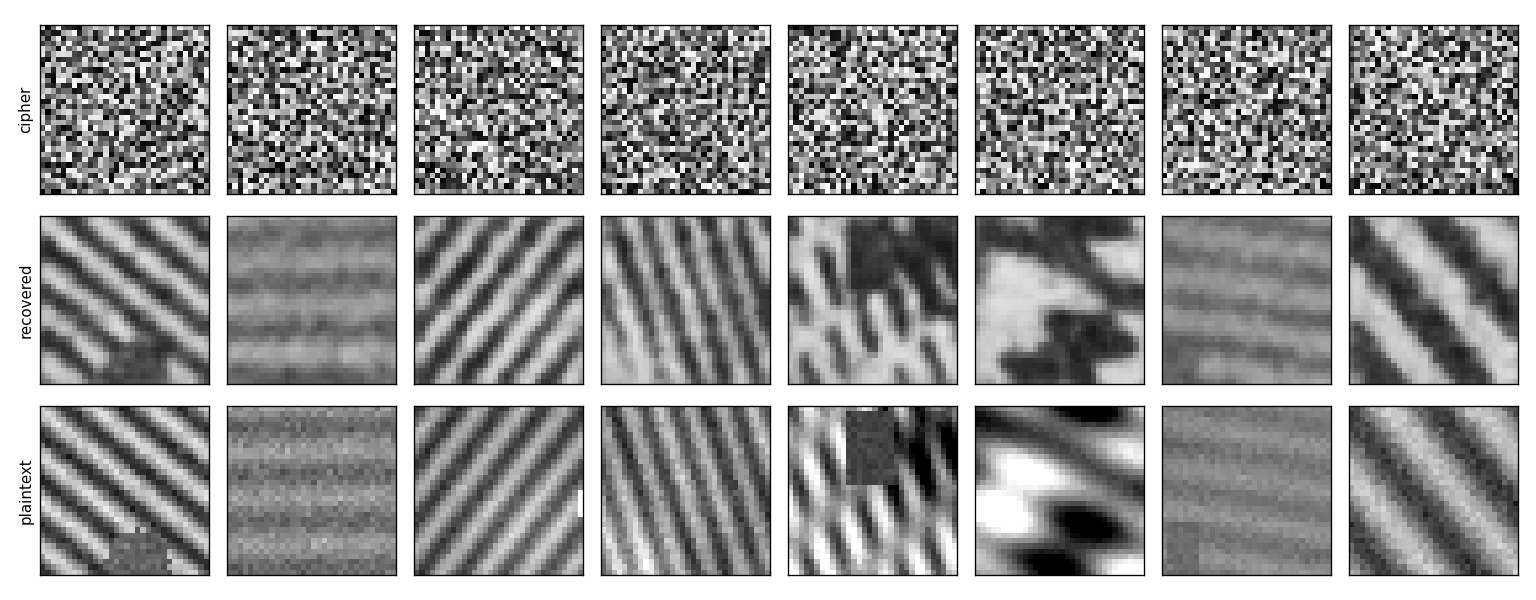
\includegraphics[width=\linewidth]{recovery-weak-chaos.png}
  \vspace{-2pt}
  \caption*{\footnotesize\color{slate}
  Weak chaos cipher. Top row: what an eavesdropper sees. Middle: the AI's
  reconstruction from that alone, no password. Bottom: the true original.}
\end{figure}

% ---------- results ----------
\section{What it shows so far}

Small proof-of-concept run (one laptop CPU, a few minutes, tiny 32\,$\times$\,32 images):

\begin{center}
\renewcommand{\arraystretch}{1.25}
\begin{tabular}{@{}l c c@{}}
\toprule
\textbf{Cipher the AI attacked} & \textbf{Image structure recovered} & \textbf{Verdict} \\
\midrule
Chaos --- value mixing only, one fixed key & \textcolor{rose}{\textbf{81\%}} & \textcolor{rose}{\textbf{HIGH}} \\
Chaos --- add pixel shuffling                & 5\%  & \textcolor{grn}{LOW} \\
Chaos --- fresh key for every image          & 5\%  & \textcolor{grn}{LOW} \\
AES-256                                       & 5\%  & \textcolor{grn}{LOW} \\
\bottomrule
\end{tabular}
\end{center}

\begin{tcolorbox}[plaincard]
The weak chaos cipher was \textbf{clearly broken} by the AI --- yet it had scored
\emph{textbook-perfect} on every classical security test (randomness 7.96 out of 8,
key-sensitivity 99.6\%, near-zero pixel correlation). \textbf{The classical tests did not
predict resistance to a learned attack.} Pixel shuffling and per-image keys are what
actually helped.

\smallskip
\textit{``Recovered'' means the picture looks similar --- not that the secret key was
extracted. That distinction is kept explicit throughout.}
\end{tcolorbox}

% ---------- done / remaining ----------
\section{Status}

\begin{tcbraster}[raster columns=2, raster equal height=rows, raster column skip=8pt]

\begin{tcolorbox}[card={Done}]
\begin{itemize}[leftmargin=1.1em]
  \item \yes Cipher library (3 chaotic maps + AES), proven reversible; 27 automated tests pass.
  \item \yes Automatic classical security profiling.
  \item \yes Data pipeline + CNN and U-Net attack models + training loop.
  \item \yes Honest scoring: improvement over a ``predict the average image'' baseline.
  \item \yes Four experiment setups: same-key, unseen-key, unseen-scheme, AES.
  \item \yes Full web app, deployable; code on GitHub with docs and a test kit.
\end{itemize}
\end{tcolorbox}

\begin{tcolorbox}[card={Remaining \& limitations}]
\begin{itemize}[leftmargin=1.1em]
  \item \gap \textbf{Scale.} Demo used tiny synthetic images on a CPU. Needs real photo
        datasets (CIFAR-10, medical, satellite) on a GPU for publishable numbers.
  \item \gap The headline break is the \emph{easiest} case (one fixed key). The key
        experiments --- does it generalise to \emph{unseen} keys and schemes --- are
        wired up but not yet run at scale.
  \item \gap Risk cut-offs (low / medium / high) are placeholders; need calibration.
  \item \gap Greyscale, square images, image encryption only, so far.
  \item \gap Back end needs its own Python host (cannot run on Vercel --- it needs PyTorch).
\end{itemize}
\end{tcolorbox}

\end{tcbraster}

\begin{tcolorbox}[plaincard]
\textbf{Next:} run the unseen-key / unseen-scheme experiments at scale on a GPU with real
datasets; add a Transformer attack model; compare against classical cryptanalysis; then
try to \emph{fix} a chaos scheme and attack it again (red-team / blue-team).
\end{tcolorbox}

\vfill
{\color{slate}\footnotesize\hrule\vspace{4pt}
Encrypted-Chaos \textbullet\ deep-learning cryptanalysis of chaos-based image encryption
\textbullet\ \href{https://github.com/ali-Hamza817/Encrypted-Chaos}{github.com/ali-Hamza817/Encrypted-Chaos}}

\end{document}
